% # COPYRIGHT:
%
% Copyright (C) 2011 Jeremiah Mahler <jmmahler@gmail.com>.
% Permission is granted to copy, distribute and/or modify this document
% under the terms of the GNU Free Documentation License, Version 1.3
% or any later version published by the Free Software Foundation;
% with no Invariant Sections, no Front-Cover Texts, and no Back-Cover Texts.
% A copy of the license is included in the file "fdl-1.3.txt".
%
\documentclass[12pt]{article}
%\usepackage{mslapa}
\usepackage{hyperref}
\usepackage{amsmath}
\usepackage{graphicx}
\usepackage{ulem}
\usepackage{vmargin}
\usepackage{tabularx}
\usepackage{sectsty}
\usepackage{pbox}
\usepackage{bigstrut}
\usepackage{enumerate}
\usepackage{parskip} % add spaces between paragraphs
\input kvmacros % Karnaugh Maps and Veitch charts
%\usepackage{cleveref}
\setpapersize{USletter}
%\setpapersize{A4}
%\setmarginsrb{<leftmargin>}{<topmargin>}{<rightmargin>}{<bottommargin>}
% {<headheight>}{<headsep>}{<footheight>}{<footskip>}
%\setmarginsrb{1.25in}{1.0in}{1.0in}{1.0in}{0in}{0.25in}{0in}{0.20in}
\setmarginsrb{1.0in}{1.0in}{1.0in}{1.0in}{0in}{0.25in}{0in}{0.20in}
\sectionfont{\normalsize}
\subsectionfont{\normalsize}
% configure \bigstrut size
% This configures spacing above and below rows in a tabularx.
%\renewcommand{\bigstrutjot}{6pt}
\renewcommand{\bigstrutjot}{2.0\jot}
\setlength{\parindent}{0in}
\raggedright
\begin{document}

% {{{ Cover Page
\centerline{\bf EECE 144}
\centerline{\bf Fall 2011}
\centerline{\bf}
\centerline{\bf Lab Report \#8}
\centerline{\bf Section 4}
\centerline{\bf 10/26/2011}
% signature area
\begin{center}
\begin{tabularx}{\textwidth}[b]{X l l}
Submitted by: Jeremiah Mahler & & \\
Signature & Printed Name & Date \\
\hline
\multicolumn{1}{|X|}{} & \multicolumn{1}{|l|}{\bigstrut \bf Jeremiah Mahler} & \multicolumn{1}{|l|}{\bf Oct 26, 2011} \\
\hline
\multicolumn{1}{|X|}{} & \multicolumn{1}{|l|}{\bigstrut \bf Marvanee Johnson} & \multicolumn{1}{|l|}{\bf Oct 26, 2011} \\
\hline
\end{tabularx}
\end{center}
% }}}

% {{{ Description/Objectives
\section{Description/Objectives}

The objective of this lab is to design circuit to implement
Equation \ref{eq:Fpos} using only a 3 to 8 line inverting
decoder ('138) and a 8 input multiplexer ('251)
\footnote{Any family of chips can be used, such as TTL (74HC) or CMOS (74LS),
but the chips from different families must not be interchanged or else
damage may result.}.
.

\begin{align}
F(a,b,c,d) 	&= \prod \; M(2,5,8,15) \label{eq:Fpos} \\
			&= M(2) M(5) M(8) M(15) \notag \\	
			&= (a' + b' + c + d')(a' + b + c' + d)(a + b' + c' + d')
				(a + b + c + d) \notag
\end{align}

% }}}

% {{{ Procedure
\section{Procedure}
\label{sec:procedure}

The truth table for the functions is given in Table \ref{tbl:tt}.
Here we are constructing a POS solution so we will only focus
on those rows with zeros (2, 5, 8, 15).
Any non-zero combination will become a 1.

\begin{table}[tbp]
\begin{center}
\begin{tabular}{lr}
\begin{tabular}[t]{r|cccc|c}
Index&$a$&$b$&$c$&$d$&$F$\\
\hline
0 &0&0&0&0 &1\\
1 &0&0&0&1 &1\\
2 &0&0&1&0 &0\\
3 &0&0&1&1 &1\\
4 &0&1&0&0 &1\\
5 &0&1&0&1 &0\\
6 &0&1&1&0 &1\\
7 &0&1&1&1 &1\\
8 &1&0&0&0 &0\\
9 &1&0&0&1 &1\\
10 &1&0&1&0 &1\\
11 &1&0&1&1 &1\\
12 &1&1&0&0 &1\\
13 &1&1&0&1 &1\\
14 &1&1&1&0 &1\\
15 &1&1&1&1 &0\\
\end{tabular}
\end{tabular}
\end{center}
\caption{Truth table of $F$ (Equation \ref{eq:Fpos}}
\label{tbl:tt}
\end{table}

This lab can be nearly impossible without a conceptual
idea of how to solve it.
The circuit to be designed should be considered a
"black box" with 4 inputs and 1 output (Figure \ref{fig:concept}).
These inputs will connect to at least one of the select
inputs on either the decoder or the multiplexer.
Since there are 4 inputs and 6 select bits between the
chips there will be unused pins.
These must be set to either high or low.

\begin{figure}[htbp]
\center
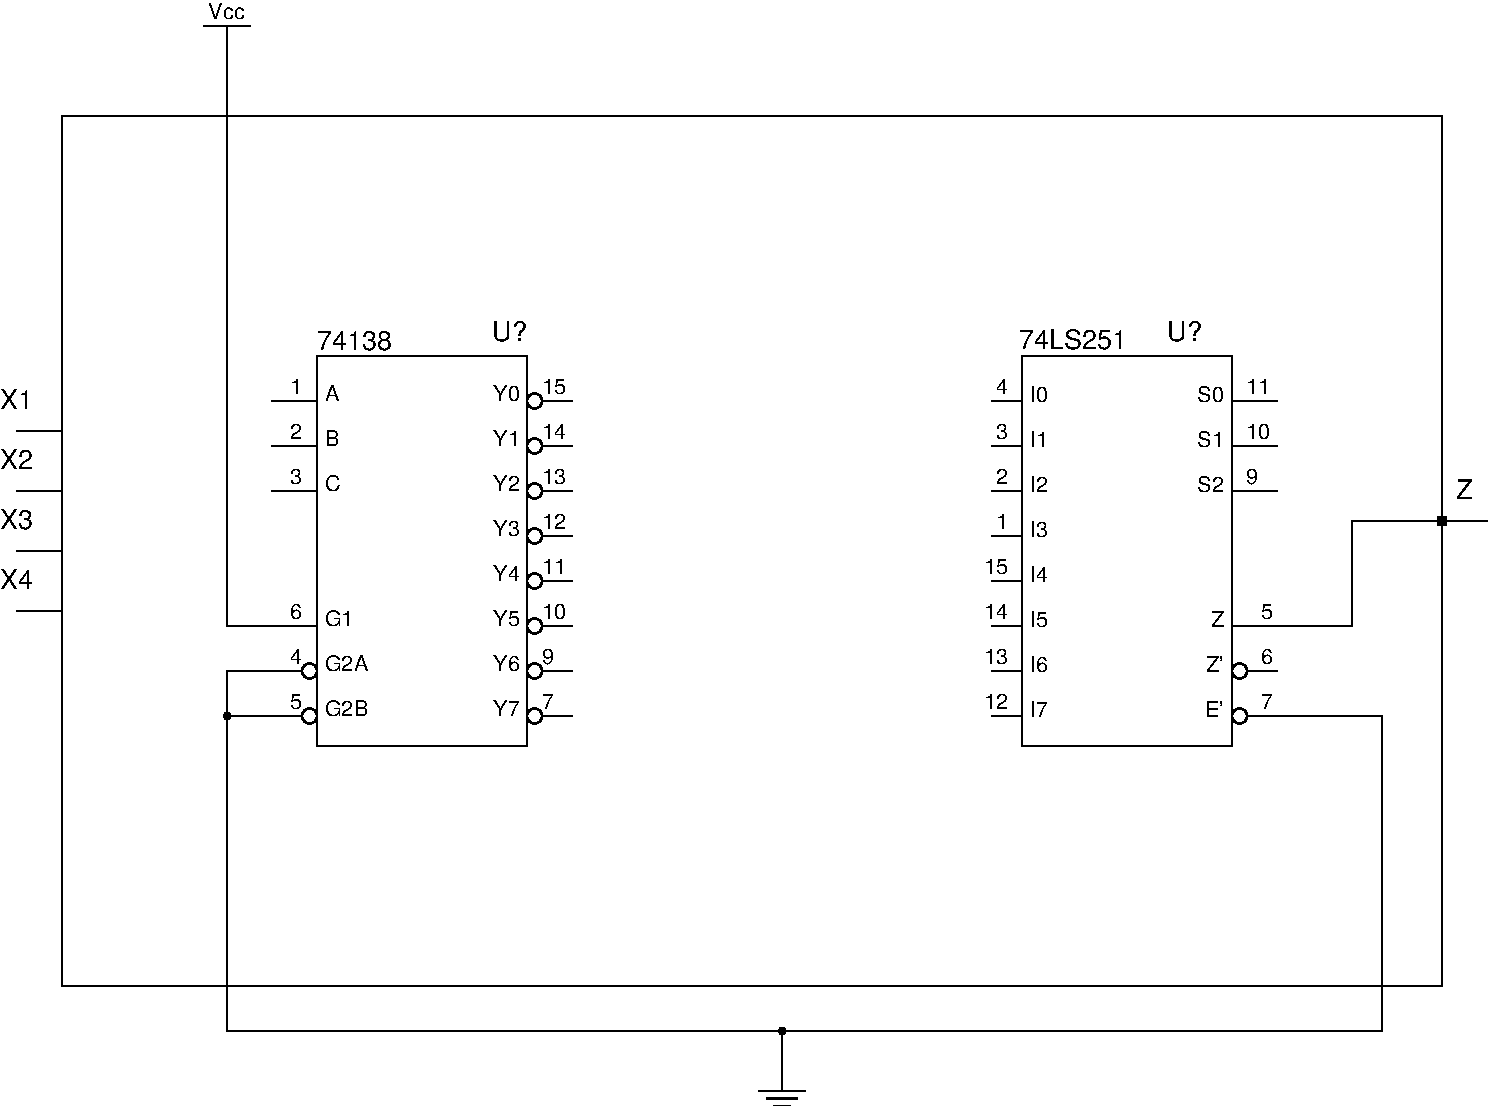
\includegraphics[scale=0.5]{lab8-circuit-01}
\caption{Conceptual design without any interconnections.  Both chips are enabled.
See Appendix \ref{sec:wksht} for a printer friendly version of this page
which can be used to solve combinations.}
\label{fig:concept}
\end{figure}

Once a combination of the outer connections to select bits 
has been chosen the next step is to find the connections
between the output bits of the decoder to the input bits
of the multiplexer.

To determine one connection, apply one of the maxterms to the
outermost inputs.
Then make a connection from the decoder to the multiplexer
such that the final output will be zero (POS).
If the connection would join together two outputs of the
decoder this is an invalid combination
\footnote{The outputs of ICs are not designed to be connected
together and doing so will most likely destroy it.}.
It is also possible that two inputs could be joined together.
Even though this would not damage the chip it is still an invalid
combination.
To try a different combination the outermost pins must be reconfigured
and the process repeated.
See Table \ref{tbl:outcon} for a listing of a few combinations.
The worksheet in Appendix \ref{sec:wksht} can be used to try out the combinations.

\begin{table}[tbp]
\begin{center}
\begin{tabular}{lr}
\begin{tabular}[t]{r|cccccc|c}
id&$A$&$B$&$C$&$S0$&$S1$&$S2$&valid?\\
\hline

0 &$X1$&$X2$&$X3$&$X4$&$0$&$0$&no\\
1 &$X1$&$X2$&$X3$&$X4$&$0$&$1$&no\\
2 &$X1$&$X2$&$X3$&$X4$&$1$&$0$&no\\
3 &$X1$&$X2$&$X3$&$X4$&$1$&$1$&no\\

4 &$X1$&$X2$&$X3$&$0$&$X4$&$0$&no\\
5 &$X1$&$X2$&$X3$&$0$&$X4$&$1$&no\\
6 &$X1$&$X2$&$X3$&$1$&$X4$&$0$&no\\
7 &$X1$&$X2$&$X3$&$1$&$X4$&$1$&no\\

8 &$X1$&$X2$&$X3$&$0$&$0$&$X4$&no\\
9 &$X1$&$X2$&$X3$&$0$&$1$&$X4$&no\\
10 &$X1$&$X2$&$X3$&$1$&$1$&$X4$&no\\
11 &$X1$&$X2$&$X3$&$1$&$0$&$X4$&no\\

12 &$X1$&$X2$&$0$&$X3$&$X4$&$0$&no\\
13 &$X1$&$X2$&$0$&$X3$&$X4$&$1$&yes\\
14 &$X1$&$X2$&$1$&$X3$&$X4$&$0$&unknown\\
15 &$X1$&$X2$&$1$&$X3$&$X4$&$1$&unknown\\

16 &$X1$&$X2$&$0$&$X3$&$0$&$X4$&no\\
17 &$X1$&$X2$&$0$&$X3$&$1$&$X4$&yes\\
18 &$X1$&$X2$&$1$&$X3$&$0$&$X4$&unknown\\
19 &$X1$&$X2$&$1$&$X3$&$1$&$X4$&unknown\\

20 &$X1$&$X2$&$0$&$0$&$X3$&$X4$&unknown\\
21 &$X1$&$X2$&$0$&$1$&$X3$&$X4$&unknown\\
22 &$X1$&$X2$&$1$&$0$&$X3$&$X4$&unknown\\
23 &$X1$&$X2$&$1$&$1$&$X3$&$X4$&unknown\\
24 & \multicolumn{6}{l|}{\ldots} & \\
?01 &$X1$&$1$&$X2$&$X3$&$1$&$X4$&yes\\
\ldots & \multicolumn{6}{l|}{\ldots} & \\
\end{tabular}
\end{tabular}
\end{center}
\caption{A few of the possible combinations of outermost connections.
Refer to Figure \ref{fig:concept} for the terminal designations.
This sample only has ordered combinations but they could be out of
order as well (e.g. $X3$ could be before $X0$).
}
\label{tbl:outcon}
\end{table}

One solved combination is shown in Figure \ref{fig:solved}.

\begin{figure}[htbp]
\center
\includegraphics[scale=0.5]{lab8-solved_circuit-01}
\caption{Solved circuit using combination with id\#13 (Table \ref{tbl:outcon}).}
\label{fig:solved}
\end{figure}

\samepage
There are several caveats to avoid when implementing this with ICs.
The encoder has three enable pins where two are inverted.
All these pins must be activated: the inverted pins should be connected
to ground and the other to $Vcc$.
The multiplexer also has an inverted enable pin that must be connected to ground.
Unused inputs to the multiplexer should be connected to $Vcc$.

\clearpage

% }}}

% {{{ Observations
\section{Observations}

There is potentially a huge number of possible combinations which
may or may not work (Table \ref{tbl:outcon}).
Only the first 20 or so combinations were examined but it would be
interesting to determine the number of possible combinations as well
as the number of valid combinations.

A working combination was found (Figure \ref{fig:solved}) and when
built using ICs it did reproduce the truth table (Table \ref{tbl:tt})
of the function (Equation \ref{eq:Fpos}).

% }}}

% {{{ Conclusion
\section{Conclusion}

With only a limited knowledge of decoders and multiplexers and without
a conceptual idea of how to design the circuit this lab was nearly
impossible.
But it was shown that is possible to build a POS equation using a decoder
and a multiplexer that would be impossible to implement with either of them
individually.

% }}}

% flush all the figures
%\clearpage
% Uncomment these if you have references,
%\pagebreak
%\renewcommand*{\refname}{\vspace{-8mm}}
%\section{References}
%%\bibliographystyle{plain}
%%\bibliographystyle{mslapa}
%\bibliographystyle{ieeetr}
%\bibliography{../references}
% Appendix (if needed)

\appendix

\clearpage
\section{Circuit Combination Worksheet}
\label{sec:wksht}

Print this page out and use it to test the various connection combinations.

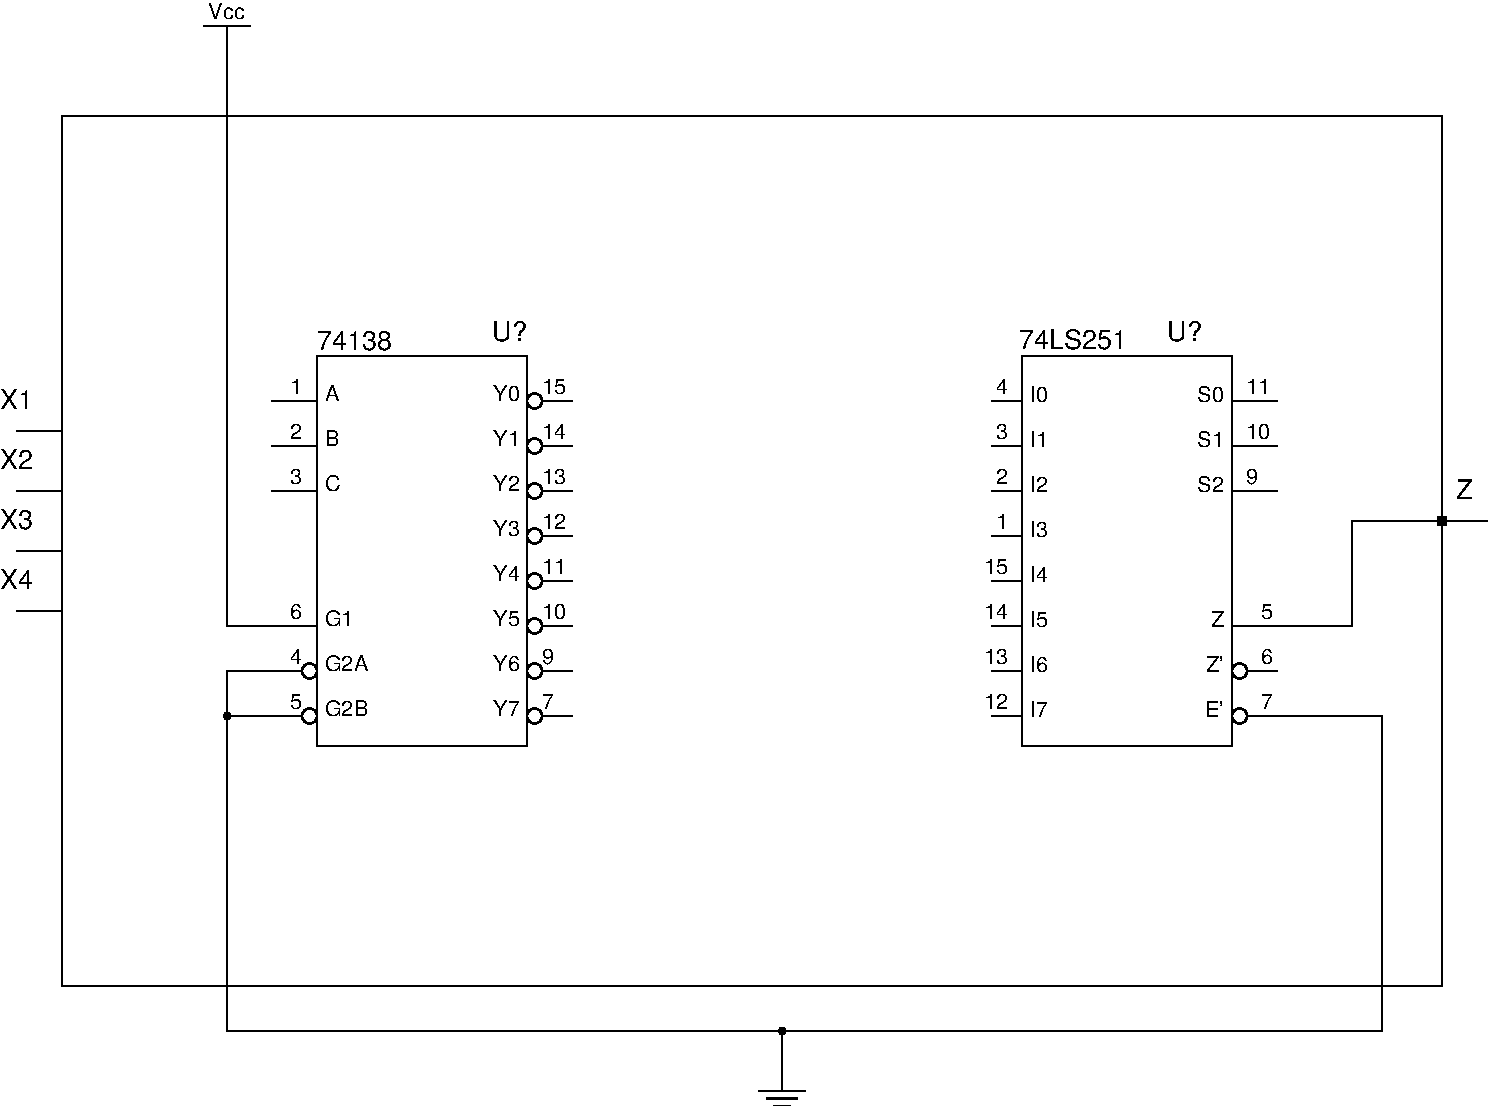
\includegraphics[scale=0.5]{lab8-circuit-01}

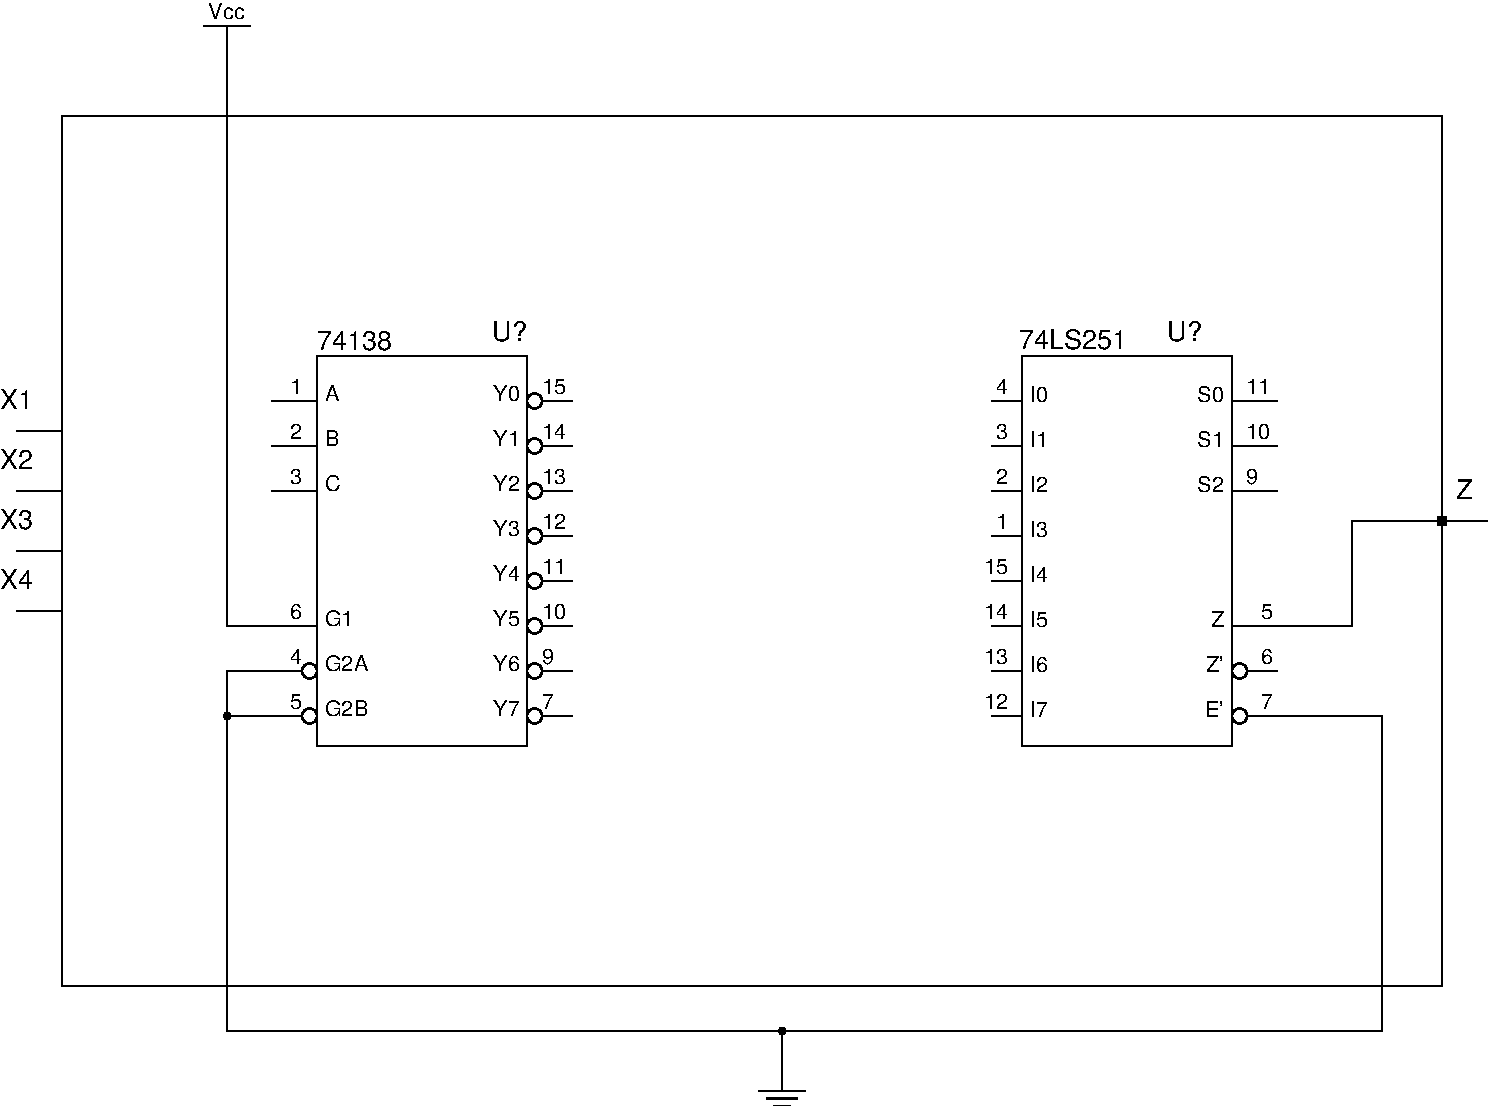
\includegraphics[scale=0.5]{lab8-circuit-01}

\end{document}

% vim:foldmethod=marker
